\begin{figure}
\centering
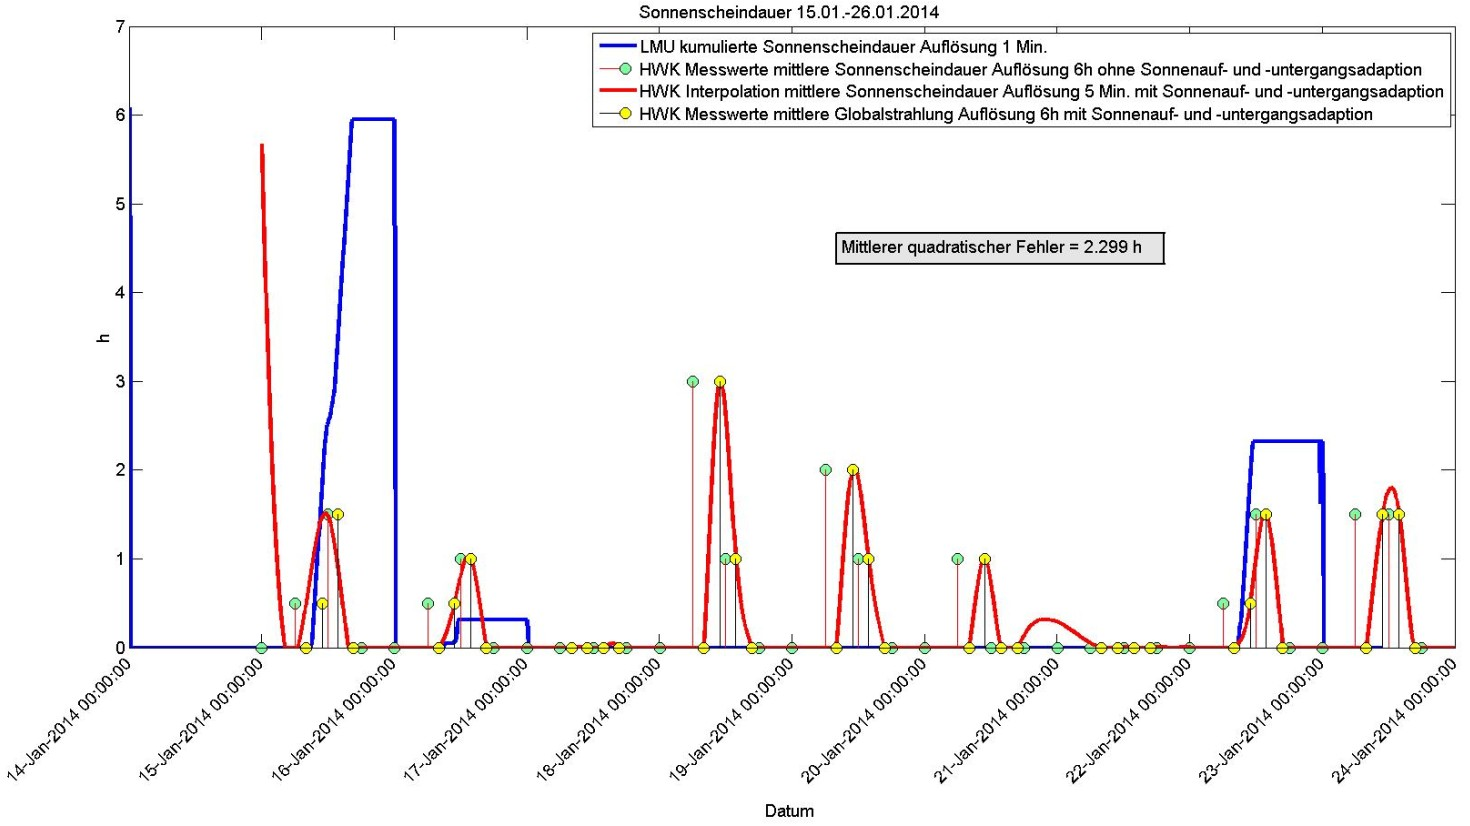
\includegraphics[width=16cm,height=10cm]{analyse/sonnensdauer2}
\caption{Vergleich der interpolierten Sonnenscheindauer mit den LMU Wetterdaten}
\label{fig:sonnensdauer}
\end{figure}

\begin{figure}
\centering
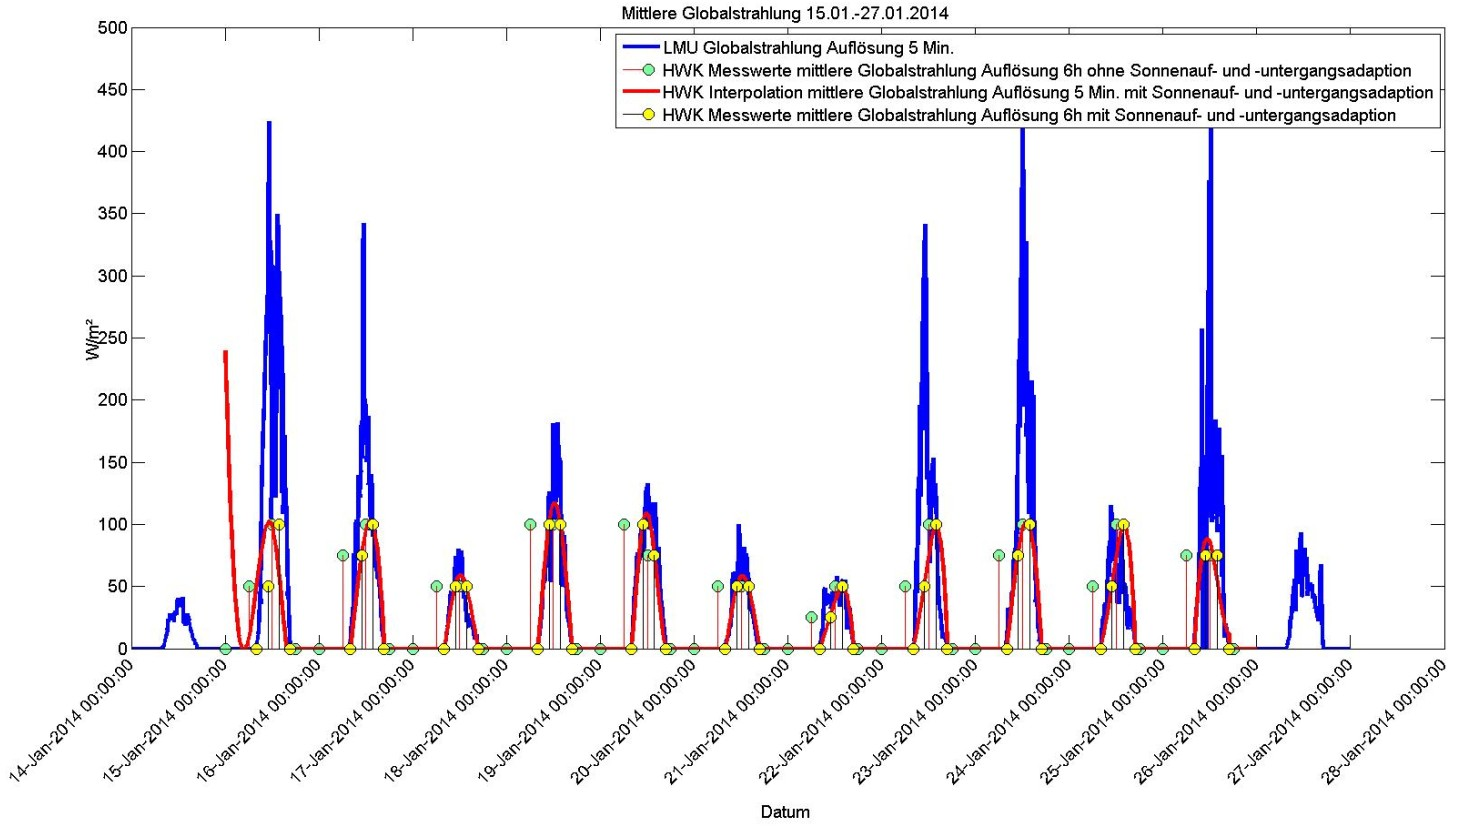
\includegraphics[width=16cm,height=10cm]{analyse/globalstr2}
\caption{Vergleich der interpolierten Globalstrahlung mit den LMU Wetterdaten}
\label{fig:globalstr}
\end{figure}
\begin{figure}
\centering
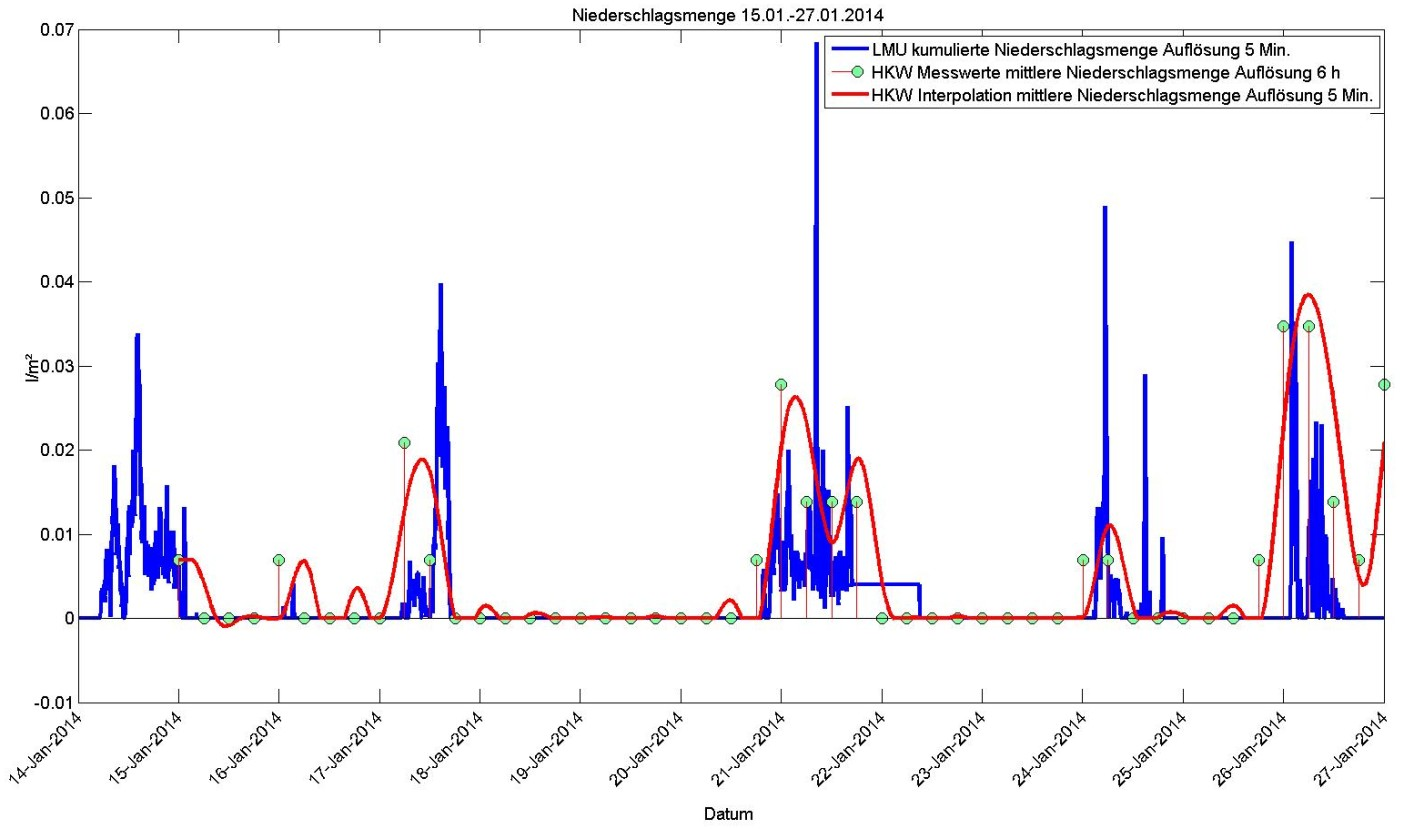
\includegraphics[width=16cm,height=10cm]{analyse/niedersmenge2}
\caption{Vergleich der interpolierten Niederschlagsmenge mit den LMU Wetterdaten}
\label{fig:niedersmenge}
\end{figure}
\begin{figure}
\centering
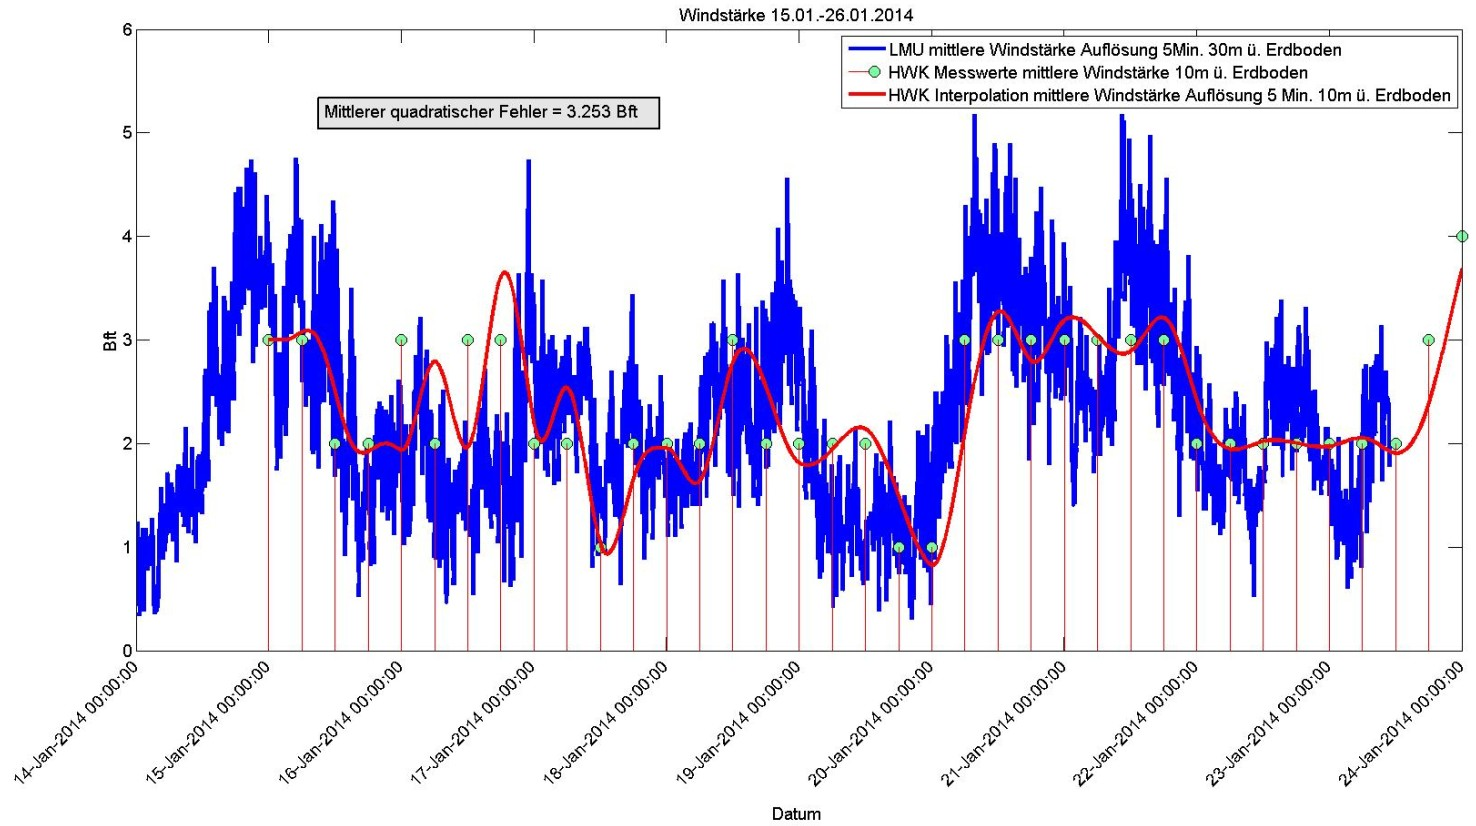
\includegraphics[width=16cm,height=10cm]{analyse/windstaerke2}
\caption{Vergleich der interpolierten Windstaerke mit den LMU Wetterdaten}
\label{fig:windstaerke}
\end{figure}
\begin{figure}
\centering
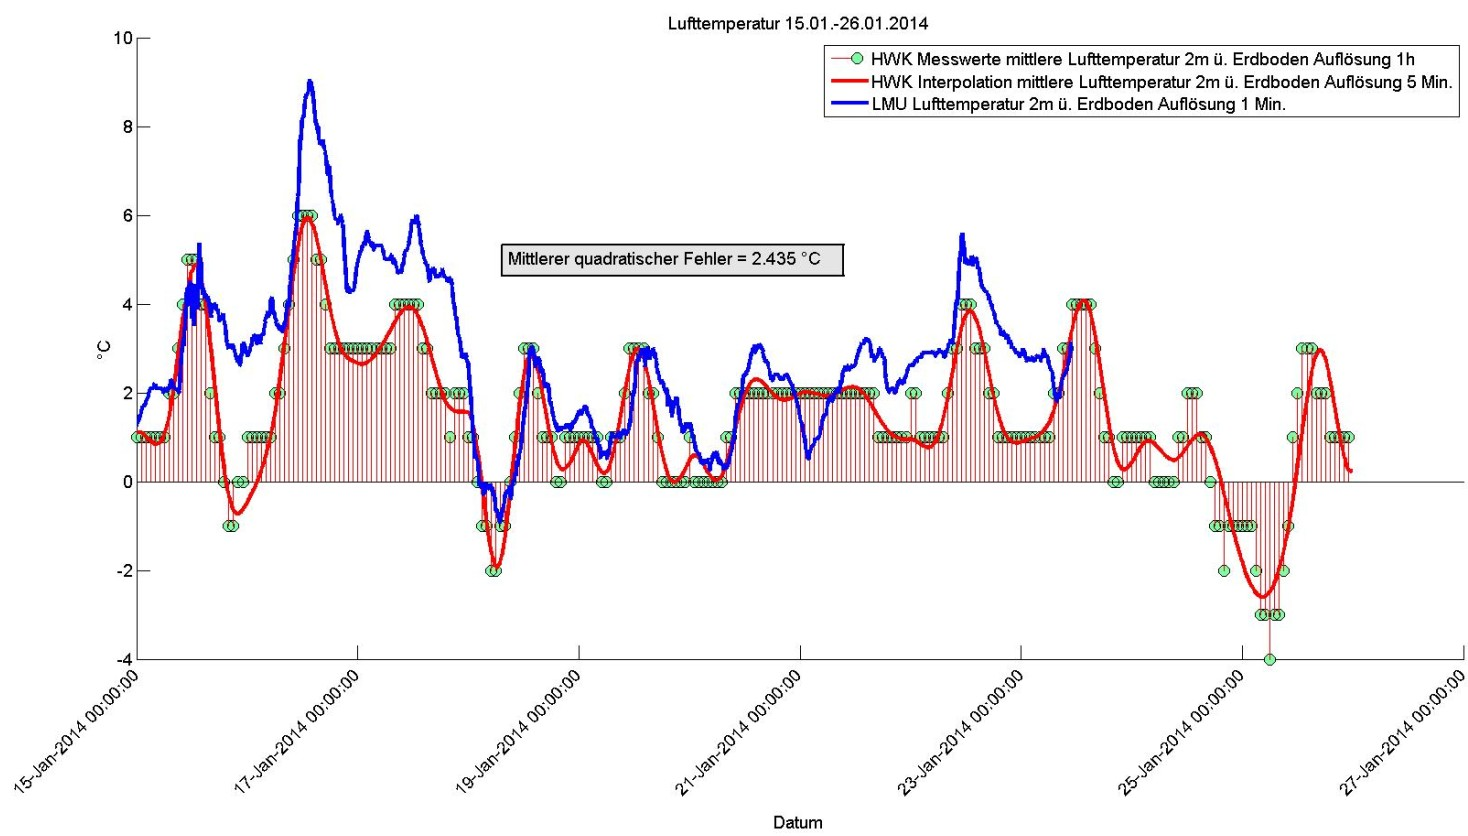
\includegraphics[width=16cm,height=10cm]{analyse/mittlufttemp2}
\caption{Vergleich der interpolierten mittleren Lufttemperatur mit den LMU Wetterdaten}
\label{fig:mittlufttemp}
\end{figure}